\documentclass{article}
\usepackage[utf8]{inputenc}
\usepackage[parfill]{parskip}
\usepackage{hyperref}
\usepackage{graphicx}
\graphicspath{ {images/} }

\usepackage{subcaption}

\title{CS394R: Programming Assignment 3}
\author{Ashish Bora}
\date{October 2016}

\usepackage{hyperref}
\hypersetup{
    colorlinks=true,
    linkcolor=blue,
    filecolor=magenta,      
    urlcolor=cyan,
}

\begin{document}

\maketitle

\section{Abstract}

In this programming assignment, we explore the Windy Gridworld problem and application of SARSA algorithm to it. We formulate the problem in the next section. In Section \ref{sarsa_alg}, we describe the SARSA algorithm and discuss why it might be an appropriate algorithm for this problem. Section \ref{impl} discusses implementation details. Finally, in Section \ref{expt}, we present several experiments, results and observations. Code used for this assignment can be found at \url{https://github.com/AshishBora/reinforcement-learning}.

\section{Introduction}

Windy Gridworld is a simple environment described in Example 6.5 in \cite{RLbook}. We briefly describe the setup here.

First, let us describe a simpler version -- the Gridworld. We will then `add' wind to it. In the Gridworld setup, there is (height $\times$ width) grid of states. In every state, the agent can take one of the four actions: move to right, left, up or down. There are walls around this grid. So trying to move through the wall results in bumping into it and hence, no movement perpendicular to the wall surface.

In Windy Gridworld, in addition to the setup above, there is an upward wind. The value of the wind in any state is the number of grid positions you move upwards, in addition to that given by the action you took, if you start from that state. Along lines of Example 6.5 from \cite{RLbook}, we only consider vertically consistent wind patterns, i.e. wind value is same for every grid point in a given column.

Given this environment, the task is to start at a given start state and reach a given goal state. The rewards are simply -1 for each time step while we have not yet reached the goal state. Thus, the goal is to reach from start state to goal state as quickly as possible. We treat this as an episodic undiscounted task.

\section{SARSA algorithm} \label{sarsa_alg}

SARSA is an online, on policy reinforcement learning algorithm. The pseudocode for the algorithm is shown in Fig. \ref{fig:sarsa}

\begin{figure}[!h]
    \centering
    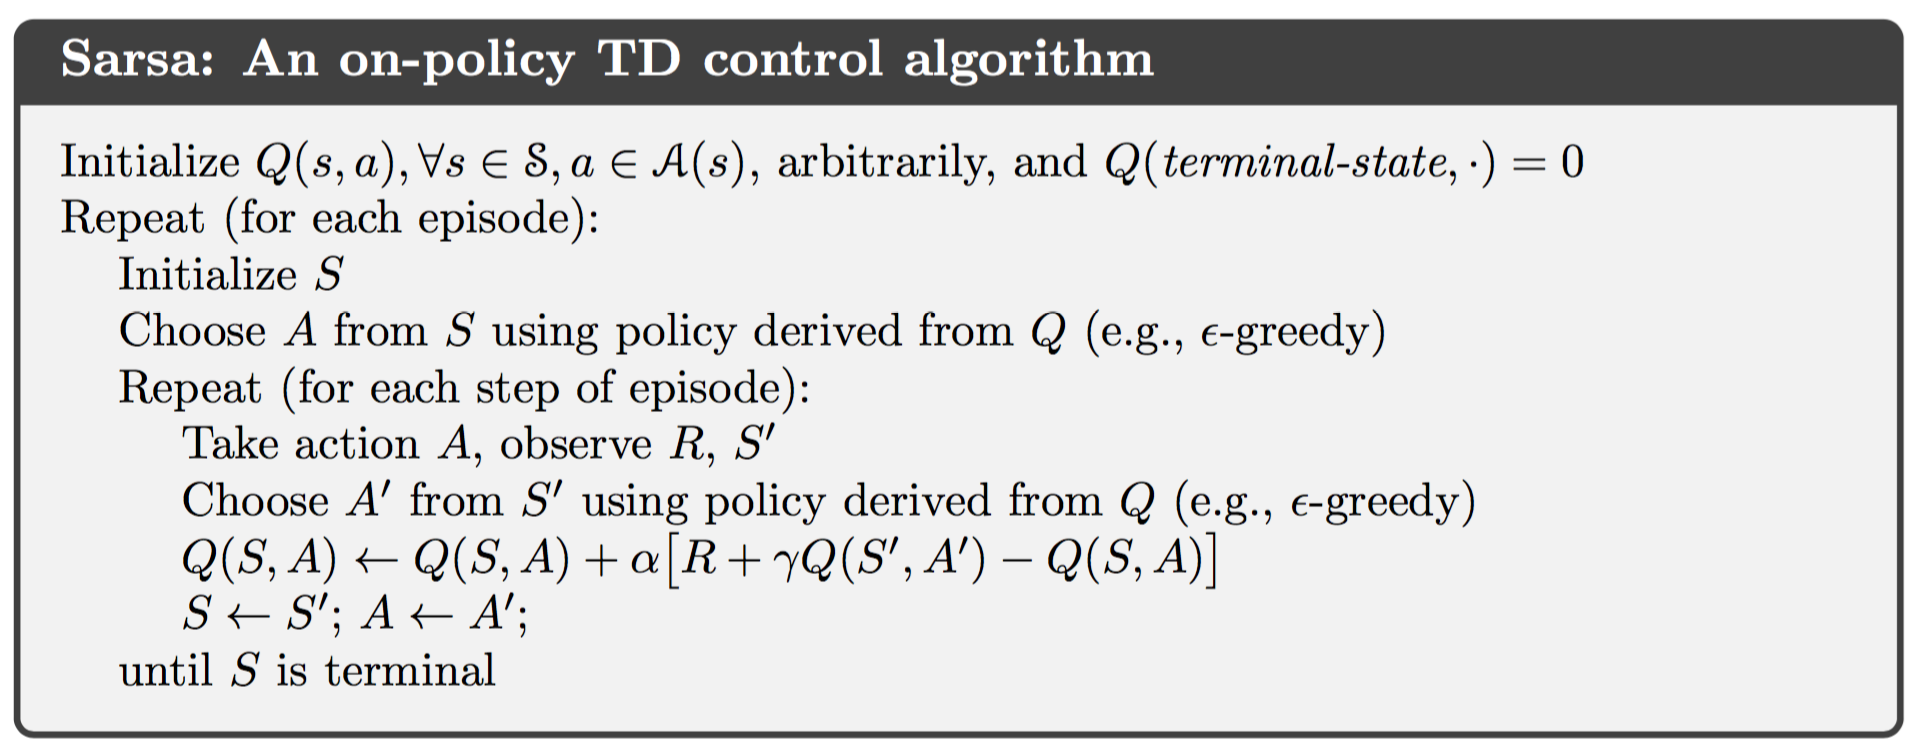
\includegraphics[width=\textwidth]{sarsa}
    \caption{SARSA algorithm. Taken from \cite{RLbook}}
    \label{fig:sarsa}
\end{figure}

Note that online learning is very useful for this task. To understand why, consider an offline algorithm like Monte Carlo. Since actions are random in the beginning, it may take forever to reach the goal state, or in the extreme case, it may not happen at all. This problem is not faced by online algorithms like SARSA since they learn-by-doing and hence can change the strategy during the episode.

\section{Implementation details} \label{impl}

The environment is implemented as a class with a step method. The agent is another class with $Q$ values as its private variables. At every step, the act method of the agent outputs the next action to take. This is then given to the environment which changes its state according to the action, and also generates a reward accordingly. The new state and the reward is communicated to the agent so that it can update its Q values. Both classes are implemented with many configurable parameters to allow easy experimentation.

We also define an experiment template. Each experiment is a list of models we want to run. Each model specifies the parameters to be used for that experiment. Then, for an experiment, each model is run and the results are plotted on the same graph for comparison.

Complete code can be found at: \\ \url{https://github.com/AshishBora/reinforcement-learning}.


\section{Experiments and Results} \label{expt}

\subsection{Expt 1}
    In this experiment, we aim to reproduce the Figure 6.4. from \cite{RLbook}. This is a simple test that our implementation is correct. We used the same setting of parameters, i.e. $\epsilon = 0.1$,  $\alpha = 0.5$ and the initial values $Q(s, a) = 0$ for all $s, a$.    
    
    We show the plot in Fig. \ref{fig:expt1}. It can be seen that we closely match the plot in Figure 6.4 from \cite{RLbook}.
    % TODO(abora) : Since sarsa involves epsilon greedy action selection which is random, we also show some uncertainty bounds around the plots.
    
    \begin{figure}[!h]
        \centering
        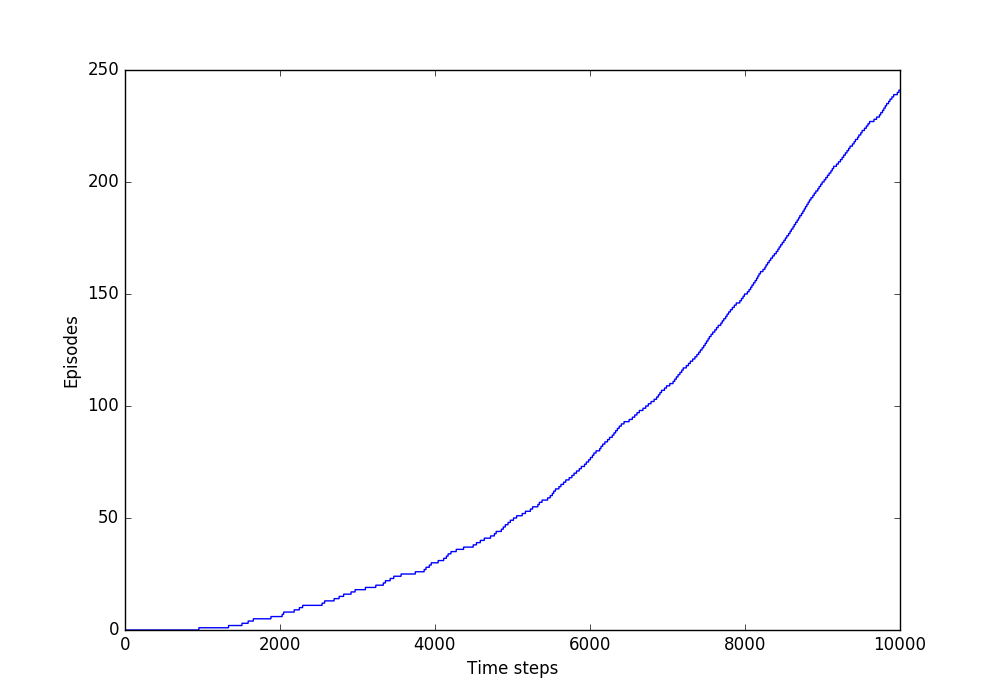
\includegraphics[width=\textwidth]{expt1}
        \caption{Experiment 1}
        \label{fig:expt1}
    \end{figure}

\subsection{Expt 2}
    In this experiment, we try to explore the paradox of choice for this problem.
    The movement up, down, right or left is always vertical or horizontal. Accordingly we call them MANHATTAN moves. Instead of MANHATTAN, we can also allow King's moves (as in chess), i.e. we are allowed to move to any of the eight neighburing states. These set of moves are denoted by KING. Going a tiny bit further, we can additionally add the ability to stay in the same place allowing for a total of nine actions. This set of moves is caleld ALL.

    Intuitively, one would think that more choice leads to better solutions. (Unfortunately, this may not be true \cite{choice}). We thus perform the experiment with the same setup, as experiment 1, to compare the three possible action sets.
    %TODO(abora) : As before, we add uncertainty bounds.
    The results are shown in Fig. \ref{fig:expt2}

    \begin{figure}[!h]
        \centering
        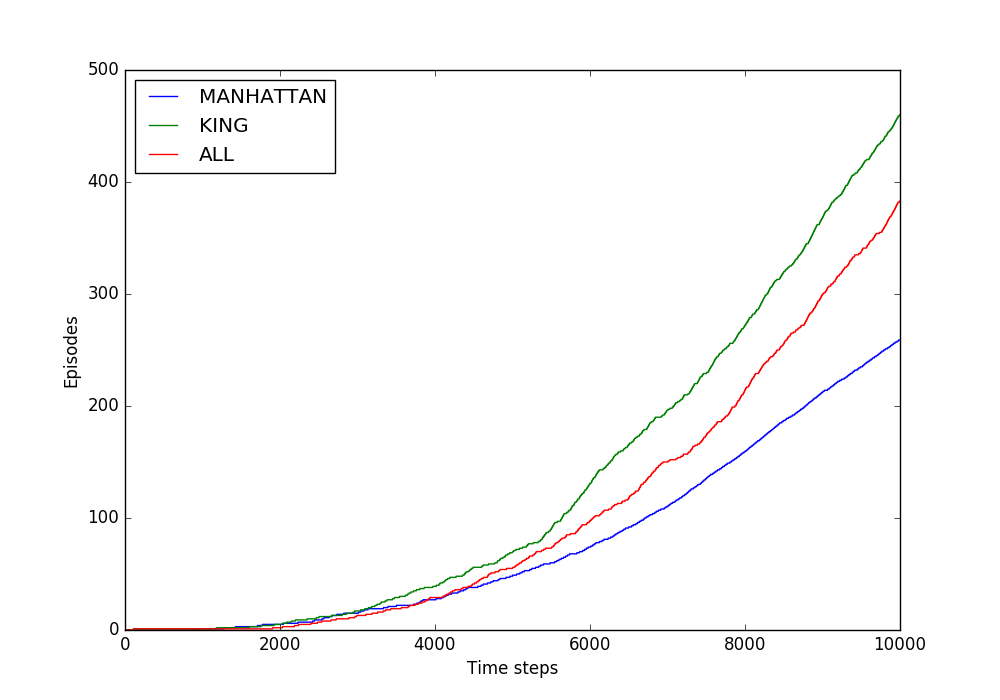
\includegraphics[width=\textwidth]{expt2}
        \caption{Experiment 2}
        \label{fig:expt2}
    \end{figure}

    From the plots, it seems that KING performs the best, followed by ALL and MANHATTAN performs the worst. One possible explanation is that since ALL moves also include staying, the model takes longer to even find a good path to the target state, thus leading to slower learning.
    
    Notice that the final slopes of the graphs for KING and ALL are very similar. This indicates that they have both learned an equally good policy by then.
    
    Also note that MANHATTEN outperforms ALL in the initial part. This is possibly because it sees more examples per action, while on the other hand, ALL has too many actions and gets confused initially. This is like bias-variance tradeoff -- with more data (which is experience, in this case), model with larger variance (ALL) becomes better than model with larger bias (MANHATTAN).


\subsection{Expt 3}
    In any reinforcement learning algorithm, having an exploring strategy is essential for visiting all states often, and thereby having a chance to learn the best policy. Accordingly, SARSA chooses actions in an $\epsilon$-greedy fashion w.r.t. to the learned $Q$ values. But since SARSA is an on-policy algorithm, unlike off-policy algorithms like $Q$-learning, its performance is affected by the amount of exploration we choose to do, i.e. by the value of $\epsilon$. In this experiment, we try to explore this relationship for the Windy Gridworld problem.
    
    We used KING's moves since that was the best model known from the previous experiment. We also kept other hyperparameters to be at the same values. The results can be seen in Fig. \ref{fig:expt3}.
    
    \begin{figure}[!h]
        \centering
        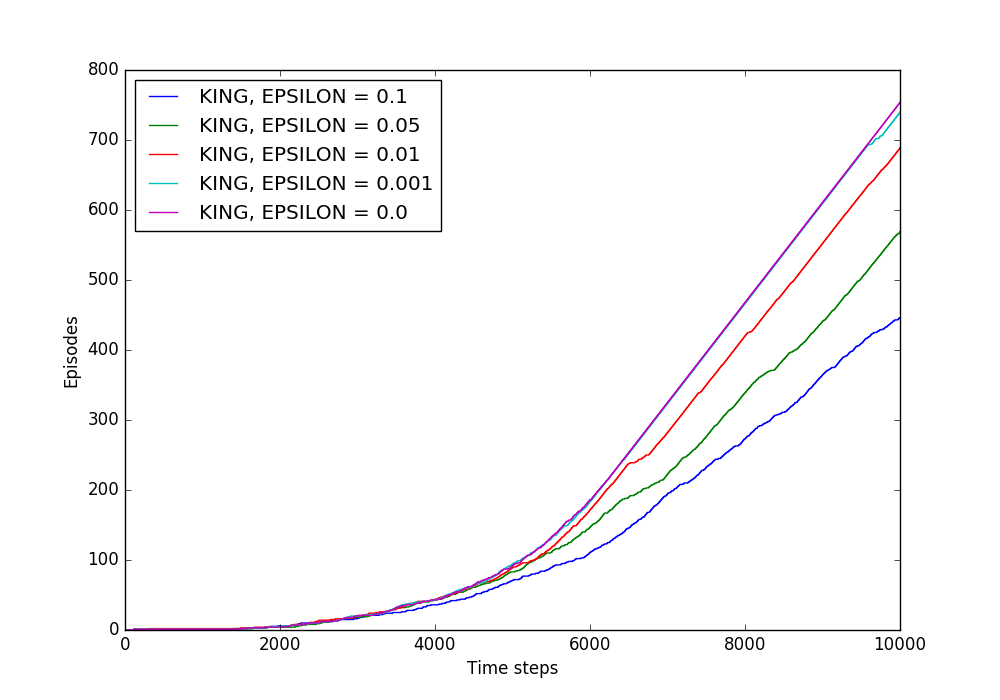
\includegraphics[width=\textwidth]{expt3}
        \caption{Experiment 3}
        \label{fig:expt3}
    \end{figure}

    From Fig. \ref{fig:expt3}, we observe that as we decrease $\epsilon$, we see substantial gains in performance.
    
    Surprisingly, the models with smaller $\epsilon$ also start performing well earlier than those with larger $\epsilon$. This is usually not true since models with larger $\epsilon$ explore more and thus find some path to the target earlier than others. This hints that $\epsilon$ is not really controlling the exploration, at least in the initial part. One possible explanation for this phenomenon is that our initialization of $Q$ values to $0$ is optimistic. This leads to exploration even for small $\epsilon$. Since all models explore well, smaller $\epsilon$ models are better able to exploit in the later half and hence get better performance eventually.
    
    Additionally, as expected, we observe that smaller $\epsilon$ models also performs better asymptotically, due to higher slopes towards the end.
    
\subsection{Expt 4}
    In this experiment, we explore a stochastic wind environment. In this case, the mean value of wind is known, but at any timestep, the wind values can be off by 1 in either direction with some probability. This probability (STOCH-PROB) is a parameter of the model . If the wind value is off from its mean, we assume that it is equally likely to be either up or down.
    
    We are interested in understanding how the performance is affected by the randomness in the environment. We emphasize that optimal amount of stochasticity is not immediately clear. Smaller stochasticity leads to better predictions by the model, but larger stochasticity leads to inherently more exploration and the model can focus on exploitation. So given a finite time horizon there is a tradeoff.
    
    Since choosing $\epsilon=0$ with KING's moves was the best for the previous experiment, we could have used it for this one as well. But $\epsilon=0$ seems a bit extreme and it might be bad if the environment itself is random. Thus we chose the next best value, $\epsilon=0.001$, since the performance of both was comparable anyway. The results are shown in Fig. \ref{fig:expt4}. 
    
    \begin{figure}[!h]
        \centering
        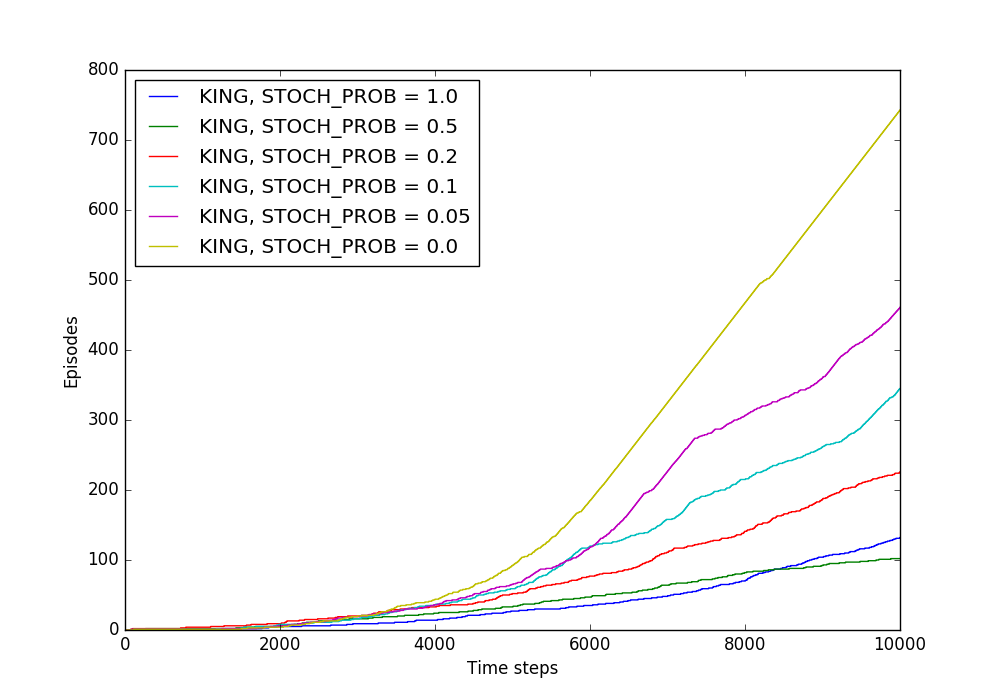
\includegraphics[width=\textwidth]{expt4}
        \caption{Experiment 4}
        \label{fig:expt4}
    \end{figure}
    
    We observet that less randomness in the environment is better for learning. A possible explanation is that optimistic initialization is forcing us explore and hence less randomness in the environment is better for learning.

\section{Conclusion}
In this assignment, we have presented the Windy Gridworld problem and applied SARSA algorithm to solve it. Then we extended the problem to include more moves and stochasticity to the transitions. In these settings, we study the performance of the algorithm with various settings of parameters.

\clearpage

\begin{thebibliography}{9}

\bibitem{RLbook}
  Richard S. Sutton and Andrew G. Barto,
  \emph{Reinforcement Learning: An Introduction},
  \url{https://webdocs.cs.ualberta.ca/~sutton/book/bookdraft2016sep.pdf}

\bibitem{choice}
  Barry Schwartz,
  \emph{The paradox of choice},
  \url{http://www.ted.com/talks/barry_schwartz_on_the_paradox_of_choice}
  
\end{thebibliography}

\end{document}